\vspace{-0.2cm}
\section{Experiments}
\label{sec:Experiments}
\vspace{-0.2cm}
%\subsection{Experimental Protocol}

We perform experiments in 6 different environments.
Implementations based on the SaLinA \citep{salina} library together with train and test environments will be released upon acceptance. For each environment, we consider one train environment on which we trained the different methods, and multiple variations of the training environment for evaluation resulting in 50 test environments in total. The details of all the environment configurations and detailed performance are given in Appendix \ref{sec:appendix_results}. Note that the complete experiments correspond to hundred of trained policies, and dozens of thousands of policy evaluations. For simple control environments (i.e., CartPole, Pendulum and AcroBot), we introduce few variations of the physics constant at test-time, for instance by varying the mass of the cart, the length of the pole. For complex control environments (i.e., HalfCheetah and Ant using the BRAX library \citep{brax2021github}, we both use variations of the physics (e.g., gravity), variations of the agent shape (e.g., changing the size of the leg, or of the foot) and sensor alterations. At last, in MiniGrid and ProcGen we perform experiments where the agent is trained in one particular levels, but is evaluated in other levels (single levels on MiniGrid, and set of 10 levels in ProcGen). Note that ProcGen is a pixel-based environment where the architecture of the policy is much more complex than in control environments.  Toy experiments on a simple Maze 2d are given in Appendix B.8 to show the nature of the policies learned by the different methods.

% \textcolor{red}{on dit nulle part quand on utilise A2C et PPO... Ca manque non ? surtout que qq part on dit deterministic/stochastic env pour le K-shot...}
We compare  our approach \textbf{LoP}\footnote{We consider the LoP-A2C and the LoP-PPO models for environments with respectively discrete and continuous actions. LoP-PPO could be also used in the discrete case but requires more hyper-parameter tuning.} with different state-of-the-art methods:
a) The \textbf{Single} approach is just a single policy learned on the train environment, and evaluated on the test ones. b) The \textbf{DIAYN+R}(reward) method is an extension of DIAYN \citep{diayn} where a set of discrete policies is learned using a weighted sum between the DIAYN reward and the task reward:
\begin{equation}
    R_{DIAYN+R}(s,a) = r(s,a) + \beta \log p(z|s)
\end{equation}
Critically, this model requires to choose a discriminator architecture to compute  $\log p(z|s)$ and modifies the train reward by defining an intrinsic reward that may drastically change the behavior of the policies at train time. c) At last, we also compare with the model proposed in \citep{Tokyo} denoted \textbf{Lc} (Latent-conditioned) that works only for continuous actions. This model is also based on a continuous $z$ variable sampled uniformly at train time, but only uses an auxiliary loss without changing the reward. This auxiliary loss is defined through the joint learning of a density estimation model $\log P(z|s,a)$ where back-propagation is made over the action $a$. As in DIAYN+R, this model needs to carefully define a good neural network architecture for density estimation. Since Lc cannot be used with environment that have discrete actions, we have adapted DIAYN+R (called \textbf{DIAYN+R Cont.}) using a continuous $z$  variable (instead of a discrete one) and a density estimation model $\log P(z|s)$ as in \cite{Tokyo}. Note that we do not compare to \citep{DBLP:conf/nips/KumarKLF20} for the exact same reason as the one identified in \citep{Tokyo}: SMERL assumes that the reward is known over the complete trajectories which results in unnatural adaptation of on-policy RL algorithms like PPO. Moreover, preliminary experiments with SMERL does not demonstrate any advantage against DIAYN+R correctly tuned. We also provide (see Table 4 in Appendix B.1) results where $K$ independent policies are learned, the best one being selected over each test environment. This approach obtains lower performance than the proposed baseline and needs $K$ more training samples making it unrealistic in most of the environments.



As network architectures, we use multi-layer perceptrons (MLP) with ReLU units for both the policy and the critic (detailed neural network architectures are described in Appendix). For DIAYN+R $\log P(z|s,...)$ is also modeled by a MLP with a soft-max output. For Lc and DIAYN+R Cont., $\log P(z|s,...)$ is modeled by a MLP that computes the mean of a Gaussian distribution with a fixed variance. For these baselines, $z$ is concatenated with the environment observation as an input for the policy and the critic models.

To choose the hyper-parameters of the different methods, let us remind that test environments cannot be used at train time for doing hyper-parameters search and/or model selection which makes this setting particularly difficult. Therefore, we rely on the following procedure:  a grid-search over hyper-parameters is made, learning a single policy over the train environment. The best value of the hyper-parameters is then selected as the one that provides the best policy at train time. These hyper-parameters are then used for all the different baselines. 
Concerning the $\beta$ value, for LoP, we report test results for $\beta=1.0$ while, for Lc and DIAYN+R, we use the best value of $\beta$ on test environments. This corresponds to an optimistic evaluation of the baseline performances; aiming at showing that our method is much more efficient since it does not need such a beta-tuning ($\beta=1.0$ giving good performance in the majority of cases). Said otherwise, we compare our model in the less favorable case where baselines have been unrealistically tuned.

For the adaptation step, each policy is evaluated over 10 episodes for stochastic environments or 1 single episode for deterministic environments. We repeat this procedure over 10 different training seeds, and report the reward over the different test environments together with standard deviation. All detailed results are available in Appendix. 

\vspace{-0.2cm}
\section{Analysis}
\label{sec:res}
\vspace{-0.3cm}
\begin{table*}[t!]
\begin{center}
\small{
\resizebox{1\linewidth}{!}{
\begin{tabular}{|l||cccc|cc|p{2cm}|p{2cm}|} \hline
& CartPole & Acrobot & Pendulum & Minigrid & Brax HalfCheetah & Brax Ant & ProcGen & toy maze   \\ 
Nb. Test Env. & 6 & 6 & 3 & 6 & 16 & 15 & 3 & 4 \\ 
Type of actions & Discr.  & Discr. & Discr.  & Discr. & Cont. & Cont. & Discr. & Discr.  \\ \hline \hline
Single Policy & 143.4& -99.7 & -52.7 & 0.169 & 7697 & 3338 & 11.09 & -83.2 \\
LoP  & 149.9& \textbf{-93.2}& \textbf{-28.9}& \textbf{0.447} & \textbf{10589} & \textbf{4031} & \textbf{16.38} & \textbf{-33.6} \\ 
DIAYN+R  &\textbf{168.1}& -97.0& -47.1& 0.248 & 9680 & 3759 & 11.45 & -42.2 \\
DIAYN+R $L_2$   &  156.1 & -93.6 & -44.0	& 0.443 & - & - & -& - \\ 
Lc   &  - &- &- 	&-  & 9547 & 4020 & -& - \\ \hline
\end{tabular}
}}
\end{center}
\vspace{-0.2cm}
\caption{Average cumulated reward of the different models over multiple testing environments averaged over 10 training seeds (higher is better). For DIAYN and Lc, we report the results %\textbf{ with  the best value of $\beta$} (this is discussed in the main text) 
and tested 10 policies for LoP, Lc and DIAYN+R using 10 episodes per policy for stochastic environments, and 1 episode per policy on deterministic ones. Performance is evaluated using the deterministic policy.  Standard deviation is reported for each single test environment in Appendix \ref{sec:appendix_results}.
}
\vspace{-0.4cm}
\label{t:all}


\label{fig:main_results}
\end{table*}

%\laure{il faut rajouter un paragraphe qq part sur l'analyse de la diversité : 1) graphique de trajectoires sur env simples discrets, 2) analyse du reward (voir fig 2c de DYIAN), 3) classifieur p(z) ou analyse nombre de skills sur halfcheetah, 4) histogramme de sélection du z en test pour dire qu'on prend pas toujours anchor et pas toujours le même}

%\laure{dans les commentaires des perfs, il faut rajouter le reward et le critère diversité (cos) en train.}


%\laure{rajouter un pragraphe sur expe in hard tasks: procgen}



We report the test performance of the models on different environments in Table \ref{fig:main_results}. %The table reports the  results obtained for the best value of $\beta$ (multiple values have been tested) which is an optimistic setting where we assume that it is possible to well tune this hyper-parameter. 
%A discussion on that point is made in the next section. 
In all the environments, the adaptive models perform better than learning a single policy over the train environment which is not surprising. In most of the cases, LoP is able to achieve a better performance than other methods. For instance, on HalfCheetah where we evaluate the different methods over 16 variations of the train environments, LoP achieves an average reward of 10589 while Lc  and DIAYN+R obtain respectively 9547 and 9680 (standard deviations are reported in Appendix \ref{sec:appendix_results}). Some examples of the discovered that behaviors in Ant and HalfCheetah\footnote{Videos available at \url{https://sites.google.com/view/subspace-of-policies/home}} for the different methods, and for different values of $z$ are illustrated in Figures \ref{fig:k-shot_ant}, \ref{fig:bigshin} and \ref{fig:hugetorso}.
This outlines that learning models that are optimal on the train task reward, but with different parameter values, allows us to discover policies react differently to variations of the training environment. It seems to be a better approach than encouraging policies to have a different behaviors (i.e., generating different state distributions) at train time. Same conclusions can be drawn in most of the environments, including MiniGrid where LoP is able to explore large mazes while being trained only on small ones. On the ProcGen environment, where the observation is an image processed through a complex ConvNet architecture (See Appendix B.7), enforcing functional diversity (DIAYN+R) does not allow to learn good policies while the LoP model is able to better generalize to unseen levels. Note that the performance at train time is the same for all the different approaches reported  (see the Table \ref{tab:beta_ablation} for instance) but quickly decreases in DIAYN for larger values of $\beta$ while it stays stable for LoP where the best results are obtained for $\beta=1.0$.

Interestingly, in CartPole, DIAYN+R performs quite well. Indeed, when analyzing the learned policies, it seems to be a specific case where it is possible to obtain optimal policies that are diverse w.r.t the states they are sampling (by moving the cart more or less on the right/left while maintaining the pole vertical). 

We have also performed experiments  where test environments have the same dynamics as the training environment, but with defective sensors (i.e., some features at test time have a null value -- see Appendix  \ref{table:ant_test_results} Table 7 on the Ant environment). The fact that LoP behaves also well confirms the effectiveness of our approach to different types of variations, including noisy features on which baselines methods were not applied in previous publications.

\begin{figure}[t!]

\hspace{0.2cm}
\begin{subfigure}{0.5\textwidth}
\small{
\resizebox{0.8\linewidth}{!}{
\begin{tabular}{ll|ccc||c|}
\multicolumn{2}{r|}{$K=$} & 5 & 10 & 20 & Train Perf.\\\midrule
 \parbox[t]{2mm}{\multirow{3}{*}{\rotatebox[origin=c]{90}{LoP}}} & $\beta=0.1$ & 3905 & 3991 & 4164  & 7659 \\
& $\beta=1.$ & \textbf{4035} & \textbf{4031} & \textbf{4174} & 7630 \\
& $\beta=10$ & 3998 & 4012 & 4145 & 7670 \\\midrule
 \parbox[t]{2mm}{\multirow{3}{*}{\rotatebox[origin=c]{90}{DIAYN}}} & $\beta=0.1$ & 3558 & 3833 & 3949 & 7739 \\
& $\beta=1.$ & 3451 & 3759 & 2878  & 5388 \\
& $\beta=10$ & 3356 & 3400 & 3109  & 4430 \\\midrule
 \parbox[t]{2mm}{\multirow{3}{*}{\rotatebox[origin=c]{90}{Lc}}} & $\beta=0.1$ & 3909 & 4020 & 4150 & 7767 \\
& $\beta=1.$ & 3820 & 3947 & 4126 & 7650  \\
& $\beta=10$ & 3870 & 3945 & 4108 & 7710 \\
 \end{tabular}
 }
 
}
\end{subfigure}
\begin{subfigure}{0.5\textwidth}
version https://git-lfs.github.com/spec/v1
oid sha256:0ff45623c53f47b1ebf41aa9cd0523ca9e45a9e32a5e7bb9fa3dc9f66605afea
size 778

\end{subfigure}
\caption{%On the left, average results obtained for different values of $\beta$ for the Ant environment averaged over 15 variations of the train environment. The right column is the 
(left) Performance of the models \textbf{at train time} that shows that for LoP $\beta$ is not hurting train performance while it is DIAYN+R. Standard error deviation is reported in Table \ref{table:ant_test_results} for each environment. We also report the performace at train time that shows that a too high value of $\beta$ hurts DIAYN+R performance while is less critical in LoP. (right) Ablation study on the number of policies $K$  used at test time on 3 HalfCheetah environment variations (see Appendix \ref{subsec:halfcheetah} for further details and additional results) together with the performance of the BoP and CoP variants. Standard deviation is given in appendix, Table \ref{table:halfcheetah_test}.}
\label{tab:beta_ablation}
    \vspace{-0.4cm}
\end{figure}

\begin{figure}[t!]

\hspace{0.2cm}
\begin{subfigure}{0.4\textwidth}
%version https://git-lfs.github.com/spec/v1
oid sha256:bf6d176fa45d8565b8ece6bdf9f6ed082b9195cad13e250472f14372a41753d6
size 358
 
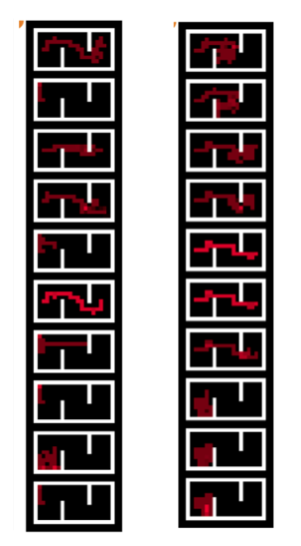
\includegraphics[width=0.75\textwidth]{images/maze.png}
\end{subfigure}
\begin{subfigure}{0.6\textwidth}
    \includegraphics[width=1.\textwidth]{images/hist_k5_halfcheetah.png}

\end{subfigure}
\vspace{-0.4cm}
\caption{(left) Trajectories generated by $K=10$ policies (one rows) on an unseen maze (objective is to go from left to right, see details in Appendix B.8) for DIAYN+R (left column with best $\beta$ value) and LoP (right column with $\beta=1.0$). It illustrates the diversity obtained with DIAYN+R and LoP. (right) Number of times (y-axis) each policy (x-axis) (over $K=5$ tested policies) is chosen over the 16 test environments of the HalfCheetah setting for each of the 10 seeds. \textcolor{blue}{Blue} is LoP and \textcolor{orange}{orange} is DIAYN+R. Different policies are used for different test environments showing the interest of learning a subspace of policies. Note that in LoP, the anchor policies are rarely chosen. Results for $K=10$ and $K=20$ in Appendix (Figure \ref{fig:histograms}).}
\label{tab:diversity}
    \vspace{-0.6cm}
\end{figure}


%\begin{table*}[t!]
%\center
%\small{
\resizebox{0.8\linewidth}{!}{
\begin{tabular}{ll|cccccc}
& &\textbf{SmallFeet} &\textbf{BigFeet} &\textbf{TinyFriction} &\textbf{HugeFriction} &\textbf{SmallGravity} &\textbf{BigGravity} \\\midrule
LoP &K=5 &8283 &\textbf{8895} &\textbf{10425} &\textbf{11537} &\textbf{11840} &\textbf{10464} \\
&K=10 &8805 &\textbf{8903} &\textbf{10662} &\textbf{11659} &\textbf{11969} &\textbf{10578} \\
&K=20 &8794 &\textbf{9096} &\textbf{10734} &\textbf{11724} &\textbf{12004} &\textbf{10807} \\\hline
DIAYN+R &K=5 &7580 &8454 &9132 &9483 &10132 &8989 \\
&K=10 &7580 &8454 &9132 &9483 &10132 &8989 \\
&K=20 &8255 &8472 &10003 &10335 &10568 &9766 \\\hline
Lc &K=5 &8186 &8353 &9521 &10305 &10434 &9360 \\
&K=10 &8186 &8340 &9661 &10379 &10444 &9488 \\
&K=20 &8107 &8431 &9661 &10505 &10521 &9506 \\\hline
BoP &K=5 &6775 &7993 &7867 &8387 &9428 &7878 \\
&K=10 &6660 &8147 &7840 &8526 &9569 &8026 \\
&K=20 &6996 &8405 &7963 &8553 &9666 &8015 \\\hline
CoP &K=5 &\textbf{8996} &8087 &9468 &10749 &10594 &9287 \\
&K=10 &\textbf{9210} &8553 &9523 &10899 &11334 &9568 \\
&K=20 &\textbf{9155} &8754 &9979 &11047 &11382 &9695 \\
\bottomrule
\end{tabular}
}
\vspace{-0.2cm}
\caption{Ablation study on the number of policies $K$  used at test time on HalfCheetah (see Appendix \ref{subsec:halfcheetah} for further details and additional results) together with the performance of the BoP and CoP variants. Standard deviation is given in appendix, Table \ref{table:halfcheetah_test}.}
}
%\vspace{-0.4cm}
%\label{tab:L_ablation}
%\end{table*}







\textbf{Sensitivity to hyper-parameters:} One important characteristic of LoP is that it can be used with $\beta=1.0$ and does not need to define any classifier architecture as opposed to DIAYN+R and Lc. Indeed, as shown in Figure \ref{tab:beta_ablation} (left), the training performance of DIAYN drastically depends on a good tuning of $\beta$. Lc, which is less sensible, needs to use a correct classifier architecture as in DIAYN. LoP is simple to tune since the cosine term is usually easy to satisfy and our approach, at convergence, always reaches a $0$ value on this term when $\beta>0.0$. As illustrated in Appendix B.1 and B2, it is also interesting to note than, on the BRAX environments, the number of environment interactions needed to train LoP is similar than the one needed to train a single policy and LoP comes with a very small overhead in comparison to classical methods.

% First of all, learning LoP is not slower than learning a single policy, and all the compared methods do not introduce any extra learning cost: we assume that it is due to the sharing of the parameters of the learned policies\footnote{In DIAYN, learning one independent policy per value of $z$ decreases the performance and learning speed.}. It means that LoP can be trained as fast as a single policy. Moreover, DIAYN+R has difficulties to reach a high training performance when the $\beta$ is high. Indeed, this model introduces an intrinsic reward that prevents the model to be optimal when the $\beta$ weight is too high. This effect is less visible in Lc and LoP that just use an auxiliary loss, but still visible on Lc whose auxiliary loss tends to modify the behavior of the policies at train time. LoP does not really suffer from high values of $\beta$ because the method is usually able to satisfy the \textit{cosine} constraint without sacrificing the train reward. In our experiment fixing $\beta=1$ always leads to a $0$ value for auxiliary term at convergence. As a confirmation, Figure \ref{tab:beta_ablation} (left) illustrates the test performance of the different methods w.r.t the weight of the auxiliary term. LoP is relatively stable whatever the value of $\beta$ and $\beta=1$ is a good and simple choice.  This is a strong point of our method: it does not need any extra hyper-parameter tuning, knowing that such a tuning is impossible when test environments are unknown. 


\textbf{Online adaptation:} One interesting property is the number of policies (and thus of episodes) to test over a new environment to get a good performance. For LoP and Lc, given a trained model, one can evaluate as many policies (i.e., different values of $z$) as desired. For DIAYN+R, testing more policies also means training more policies which is expensive and less flexible. Table \ref{tab:beta_ablation} (right) provides the reward of the different methods when testing $K$ policies on different HalfCheetah settings: as expected, the performance of DIAYN+R tends to decrease when $K$ is large since the model has difficulties to learn too many diverse policies. For LoP and Lc, spending more episodes to evaluate more policies naturally leads to a better performance: these two models provide a better way to deal with the exploration-exploitation trade-off at test time. Again, please consider that Lc also needs to define an additional neural network architecture to model $\log P(z|s,a)$ while LoP does not, making our approach simpler.% \laure{voir le commentaire sur K=0 et augmenter K}

\textbf{Beyond a Line of Policies: } While LoP is based on the learning of $N=2$ anchor parameters, it is possible to combine more than two anchor parameters. We study two approaches combining $N=3$ anchor parameters (that can be extended to $N=3$): a) the first approach is a convex combination of policies (CoP) where $z$ is sampled following a Dirichlet distribution. (b) The second approach is a Bézier combination (BoP) as explained in Appendix \ref{subsec:bopcop}. The results are presented in Table \ref{tab:beta_ablation} (right) over multiple HalfCheetah environments. It can be seen that these two strategies are not so efficient. LoP is thus a good trade-off between the number of parameters to train and the performance (Note that BoP and CoP need more samples to converge), at least given the particular neural network architectures we have used in this paper. We also performed an in-depth analysis of the evolution of the reward when K is increasing for LoP and CoP in Halfcheetah test environment (Figure \ref{fig:K_evolution} in Annex). While we expected CoP to outperform LoP when K is high, the best reward becomes stable when K=20 for both methods, and in most test environments, CoP is not able to reach the same best reward as LoP. %\laure{commentaire sur K qui augmente croisé au N=3, peut-être plsu d'augmentation pour N=3 alors qu'avec N=2, il satures} 



\textbf{Analysis of the learned policies: } To better understand the nature of the policies discovered by the different approaches, we have made a qualitative study in which we analyze i) the robustness of the methods to corrupted observations, ii) the functional diversity induced by the different models, and iii) the specificity of the different learned policies to particular test environments. First, LoP is more robust to input feature corruption (see Table \ref{table:ant_test_results} for the results, and Table \ref{table:ant_test_setting} for the setting in Appendix) and we conjecture that it is because the diversity in the parameter space allows this model to learn policies that does not take into account the same input features equally. We also measure the functional diversity induced by the different models by training \textit{a posteriori} a classifier that aims at recovering which policy (i.e which value of $z$) has generated particular trajectories (Exact protocol in Figure \ref{fig:discriminator_accuracy} in Appendix, with the training curves). On LoP with $K=5$, such a classifier obtains a 82\% accuracy at validation time showing that the $5$ policies are quite diverse, but less than the DIAYN+R policies where the classifier reaches a 100\% accuracy which is logical knowing the auxiliary loss introduced by DIAYN which enforces this type of diversity. It is interesting to note that with the trajectories generated in the test environments with LoP policies, the accuracy of the classifier is reaching 87 \%: when LoP is facing new environments, it tends to generate more diverse policies. We think that it is due to the fact that, since the policies have different parameter values, they react differently to states that have not been encountered at train time.  At last, Figure 4 (right) (and Figure 7 in appendix for K=10,20) illustrates which upon $K=5$ policies is used for different test environments. It shows that both LoP and DIAYN+R use different policies over different test environments, showing that these methods are able to solve new environments by learning various policies and not a single but robust one. Examples of policies on a simple maze2d are given in Figure \ref{tab:diversity} (left) and Appendix which illustrate the diversity of the discovered policies.


%\textbf{Analysis of the diversity learned:} \textcolor{violet}{JB : Point 1 discriminator learned (details of the experiments in appendix) : in order to see how our method compare to skill discovery methods, we tried to learn a discriminator from scratch with a dataset of trajectories collected by sampling learned policies. For each environment, and for each seed, a different discriminator is learned and the accuracy is computed on a validation set and averaged. \\ \\ Point 2 Histogram : we performed an in-depth analysis of the distribution of the policies used at test time. For each seed of the models learned on halfcheetah, we plot the number of times a policy is chosen after k-shot evaluation. (see appendix XXX for other results for k=10, k=20). We can see that for k=5, at least 3 policies are useful, always the policies in the middle are chosen. the Results for k=10 are similar. 
%IMPORTANT : say that for beta = 10 DIAYN histograms are way more peaked. i.e. beta = hard to tune} 

%\begin{figure}[t]
%\begin{subfigure}{0.5\textwidth}
%    \includegraphics[width=1.0\textwidth]{images/bezier_halfcheetah.png}
%    \caption{Performance at train time w.r.t environment interactions. %With the same hyper-parameters as LoP, CoP reaches similar %performance, while BoP improvement is much slower, suggesting that a %bit of fine-tuning of $\beta$ might be  necessary. \textcolor{red}{A %virer si features bruitees fonctionne}}
 %   \label{fig:learn_bezier}
%\end{subfigure}
%\hspace{0.2cm}
%\begin{subfigure}{0.5\textwidth}
%\begin{tabular}{ll|ccc}
& &\textbf{HalfCheetah}  \\\midrule
LoP ($N=2$) &K=5 & 9889  \\
&K=10 & 10032  \\
&K=20 & 10119  \\ \hline
BoP ($N=3$)&K=5 & 8254 \\
&K=10 & 8331  \\
&K=20 & 8453  \\ \hline
CoP ($N=3$)&K=5 & 9514 \\
&K=10 & 9781  \\
&K=20 & 9990  \\ \hline
\end{tabular}

%\caption{Rewards averaged over the 16 Halfcheetah test environments. }
%\label{tab:bezier_study}
%\end{subfigure}
%\center
%\vspace{-0.4cm}
%\caption{HalfCheetah performance with LoP, CoP and BoP. Results are %averaged over 10 seeds.}
%\vspace{-0.4cm}
%\label{fig:shapeSubspace}
%\end{figure}






